\documentclass[crop,convert={convertexe={magick},outext=.png}]{standalone}

% Tikz
\usepackage{pgfplots,pgfplotstable}
\usepackage{amsfonts}
\usepackage{tikz}
\pgfplotsset{compat=1.18}

\begin{document}

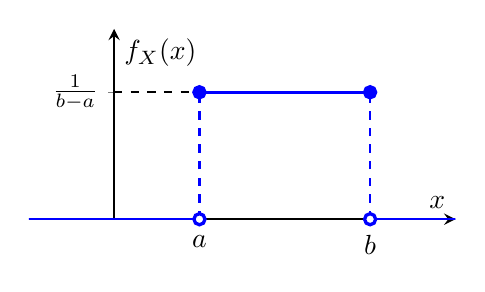
\begin{tikzpicture}[
    declare function={unipdf(\x,\xl,\xu)= (\x>=\xl)*(\x<\xu)*1/(\xu-\xl);}
]
\pgfplotsset{soldot/.style={color=blue,only marks,mark=*}} \pgfplotsset{holdot/.style={color=blue,fill=white,only marks,mark=*}}
\begin{axis}[
	height=4cm,width=7cm,xlabel={$x$}, ylabel={$f_X(x)$},axis lines=middle, 
	thick,legend pos=outer north east,
    samples=1000,
    ymin=0,ymax=1.5,
    xmin=-0.5, xmax=2, 
    xtick={0.5,1.5},
    ytick={1},
    xticklabels={$a$,$b$},
    yticklabels={$\frac{1}{b-a}$},
    jump mark left,
    every axis plot/.style={very thick}
%    discontinuous
]
\addplot [blue,jump mark left] {unipdf(x,0.5,1.5)};
	\draw[dashed,blue] (axis cs:0.5,0) -- (axis cs:0.5,1);
	\draw[dashed,blue] (axis cs:1.5,0) -- (axis cs:1.5,1);
\draw[dashed,black] (axis cs:0,1) -- (axis cs:0.5,1);	
\addplot[holdot] coordinates{(0.5,0)(1.5,0)};
\addplot[soldot] coordinates{(0.5,1)(1.5,1)};
\end{axis}
\end{tikzpicture}

\end{document}